\hypertarget{test__replace2_8cpp}{}\subsection{test\+\_\+replace2.\+cpp File Reference}
\label{test__replace2_8cpp}\index{test\+\_\+replace2.\+cpp@{test\+\_\+replace2.\+cpp}}


Contains an example to take subject string, replacement string, modifier and pattern from user input and perform regex replace with J\+P\+C\+R\+E2.  


{\ttfamily \#include $<$iostream$>$}\\*
{\ttfamily \#include \char`\"{}jpcre2.\+hpp\char`\"{}}\\*
Include dependency graph for test\+\_\+replace2.\+cpp\+:\nopagebreak
\begin{figure}[H]
\begin{center}
\leavevmode
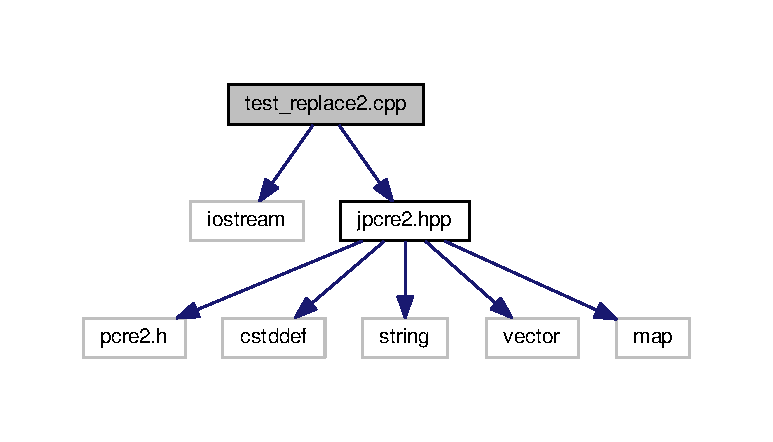
\includegraphics[width=350pt]{test__replace2_8cpp__incl}
\end{center}
\end{figure}


\subsubsection{Detailed Description}
Contains an example to take subject string, replacement string, modifier and pattern from user input and perform regex replace with J\+P\+C\+R\+E2. 


\begin{DoxyCodeInclude}
\textcolor{comment}{/**@file test\_replace2.cpp}
\textcolor{comment}{ * Contains an example to take subject string, replacement string, modifier and pattern}
\textcolor{comment}{ * from user input and perform regex replace with JPCRE2}
\textcolor{comment}{ * @include test\_replace2.cpp}
\textcolor{comment}{ * @author [Md Jahidul Hamid](https://github.com/neurobin)}
\textcolor{comment}{ * */}


\textcolor{preprocessor}{#include <iostream>}
\textcolor{preprocessor}{#include "\hyperlink{jpcre2_8hpp}{jpcre2.hpp}"}


\textcolor{preprocessor}{#define getLine(a) std::getline(std::cin,a,'\(\backslash\)n')}


\textcolor{keywordtype}{int} main()\{
    std::string pat,mod,subject,repl,repl\_mod;

    std::cout<<\textcolor{stringliteral}{"\(\backslash\)nEnter pattern: "};
    getLine(pat);

    std::cout<<\textcolor{stringliteral}{"\(\backslash\)nEnter compile modifiers (eijmnsuxADJSU): "};
    getLine(mod);
    \hyperlink{classjpcre2_1_1Regex}{jpcre2::Regex} re;     \textcolor{comment}{/// This is not supposed to throw any exception.}
\textcolor{comment}{}
\textcolor{comment}{}
\textcolor{comment}{    /// Compile the pattern}
\textcolor{comment}{}    \textcolor{keywordflow}{try}\{re.\hyperlink{classjpcre2_1_1Regex_aad1d5ef1e87f762f68a587eec4022e69}{compile}(pat,mod);\}
    \textcolor{keywordflow}{catch}(\textcolor{keywordtype}{int} e)\{std::cerr<<re.\hyperlink{classjpcre2_1_1Regex_a92b75c438ccff871205b2175a6141fd5}{getErrorMessage}(e);\}


    \textcolor{comment}{/******************************************************************************************************
      *********}
\textcolor{comment}{     * Use try catch block to catch any exception and avoid unexpected termination of the program in case
       of error.}
\textcolor{comment}{     * All jpcre2 exceptions are of type int (integer)}
\textcolor{comment}{     * ****************************************************************************************************
      *********/}

\textcolor{comment}{}
\textcolor{comment}{    ///subject string}
\textcolor{comment}{}    std::cout<<\textcolor{stringliteral}{"\(\backslash\)nEnter subject string (enter quit to quit): "}<<std::endl;
    getLine(subject);
    \textcolor{keywordflow}{if}(subject==\textcolor{stringliteral}{"quit"})\textcolor{keywordflow}{return} 0;\textcolor{comment}{}
\textcolor{comment}{     ///replacement string}
\textcolor{comment}{}    std::cout<<\textcolor{stringliteral}{"\(\backslash\)nEnter replacement string: "}<<std::endl;
    getLine(repl);
\textcolor{comment}{}
\textcolor{comment}{    /// Continue loop as long as error occurs}
\textcolor{comment}{}    \textcolor{keywordflow}{while}(\textcolor{keyword}{true})\{
        std::cout<<\textcolor{stringliteral}{"\(\backslash\)nEnter action (replacement) modifiers (eEgx): "};
        getLine(repl\_mod);

        \textcolor{comment}{//perform replace}

        \textcolor{keywordflow}{try}\{std::cout<<\textcolor{stringliteral}{"\(\backslash\)nreplaced string: "}<<re.\hyperlink{classjpcre2_1_1Regex_ae7235a991492fa88f1bd3fb02d59cd0a}{initReplace}()
                                                .\hyperlink{classjpcre2_1_1RegexReplace_a46eefdb105827920bebc8436721fa4cb}{setSubject}(subject)
                                                .\hyperlink{classjpcre2_1_1RegexReplace_af1069f489de9b343493da2dc77b04c73}{setReplaceWith}(repl)
                                                .\hyperlink{classjpcre2_1_1RegexReplace_ae2abe2994b0fbe54950f88e63000c910}{setModifier}(repl\_mod)
                                                .\hyperlink{classjpcre2_1_1RegexReplace_a3f86b1e11d08d0153a08244771e59061}{addJpcre2Option}(
      \hyperlink{namespacejpcre2_a85c143271501e383843f45b9999c2f00a9124b768bcae4d51430aa7f26126f387}{jpcre2::VALIDATE\_MODIFIER})
                                                .\hyperlink{classjpcre2_1_1RegexReplace_afd087fa7a9bfedec802d1a3dd7edbdd0}{replace}();\}
        \textcolor{keywordflow}{catch}(\textcolor{keywordtype}{int} e)\{std::cerr<<re.\hyperlink{classjpcre2_1_1Regex_a92b75c438ccff871205b2175a6141fd5}{getErrorMessage}(e);
            \textcolor{keywordflow}{if}(e==\hyperlink{namespacejpcre2_1_1ERROR_a4b2998984439438fa9da8d7043909bc2a4115340549b623f4e2da285bf0aa9bff}{jpcre2::ERROR::INVALID\_MODIFIER}) \textcolor{keywordflow}{continue};
        \}
        \textcolor{keywordflow}{break};
    \}
    std::cout<<\textcolor{stringliteral}{"\(\backslash\)n\(\backslash\)n--------------------------------------------------\(\backslash\)n"};
    \textcolor{comment}{//main();}
    \textcolor{keywordflow}{return} 0;
\}
\end{DoxyCodeInclude}
 \begin{DoxyAuthor}{Author}
\href{https://github.com/neurobin}{\tt Md Jahidul Hamid} 
\end{DoxyAuthor}
